
% to choose your degree
% please un-comment just one of the following
\documentclass[bsc,frontabs,twoside,singlespacing,parskip,deptreport]{infthesis}     % for BSc, BEng etc.
% \documentclass[minf,frontabs,twoside,singlespacing,parskip,deptreport]{infthesis}  % for MInf


\usepackage{graphicx}
\begin{document}

\title{Implementing an online open-source prediction market framework}

\author{Yordan Stoyanov}

% to choose your course
% please un-comment just one of the following
%\course{Artificial Intelligence and Computer Science}
%\course{Artificial Intelligence and Software Engineering}
%\course{Artificial Intelligence and Mathematics}
%\course{Artificial Intelligence and Psychology }   
%\course{Artificial Intelligence with Psychology }   
%\course{Linguistics and Artificial Intelligence}    
%\course{Computer Science}
\course{Software Engineering}
%\course{Computer Science and Electronics}    
%\course{Electronics and Software Engineering}    
%\course{Computer Science and Management Science}    
%\course{Computer Science and Mathematics}
%\course{Computer Science and Physics}  
%\course{Computer Science and Statistics}    

% to choose your report type
% please un-comment just one of the following
%\project{Undergraduate Dissertation} % CS&E, E&SE, AI&L
%\project{Undergraduate Thesis} % AI%Psy
\project{4th Year Project Report}

\date{\today}

\abstract{
Model aggregation, markets, prediction markets. 

My market
}

\maketitle

\section*{Acknowledgements}
You guys have been a great inspiration!

\tableofcontents

%\pagenumbering{arabic}


\chapter{Introduction}

Information has been traded extensively in one way or another since the dawn of man. While true, this fact has become increasingly relevant in recent years with advances such as the information economy and big data transforming the way we think about data and the knowledge it implies \cite{mcgee_managing_1993}; at the same time it has never been harder to quantify its value. 


The problem of efficiently combining information coming from different sources in order to form a rational belief is largely an unsolved issue in Bayesian philosophy \cite{greene_collective_2010}. It manifests in the domain of machine learning as the problem of belief aggregation which deals with the design of algorithms that combine the beliefs of multiple {\em weaker} learners in order to elicit a stronger, more accurate belief. In practice though existing solutions are 

	If we take a look at ordinary commodity trading though it is apparent that the existence of a market where agents exchange goods using a common currency provides a meaningful way to determine the prices of the traded goods. Note that while the traded goods can be physical, it is often the case that they are purely conceptual. For example the prices of stock market shares reflect the public's expectation of the performance of a company in the near future. The basic market needs not be active with regard to the traded goods and is in principle nothing more than the market squares that have existed in towns for ages. In its essence a market provides the basic process for determining the price, demand and ownership of various goods or services. 

	A prediction market is a special kind of a market which allows agents to trade on and share their information on a future event with the public. This is achieved by creating a market where the trading goods are akin to shares corresponding to each of the possible outcomes of the events of interest. Each share promises a fixed payment in the future to its holder if and only if the outcome associated with it happens to be the event's actual result. This future point is usually fixed at the start of each challenge, necessarily after the result of the event has been observed by the public. In such a way players are incentivised to trade on the difference between their beliefs and those of the market: rational agents would buy shares at what they perceive to be a lower price as this increases their expected profit. By doing so they practically inform the market and the public of their knowledge and help establish the equilibrium price. 

	Another possible application of prediction markets deals with the creation of crowdsourced machine learning competitions. Such challenges have become popular. The main motivation behind such approaches is to leverage the knowledge of the public at scale by offering incentives for the interested and knowledgeable parties. A prominent example is the {\em Netflix prize} challenge which was held with a recognised success as early as 2006 with the goal of improving the classification algorithms used by the company\cite{bennett_netflix_2007}. The online platform {\em Kaggle} takes a slightly different approach by instead hosting such competitions on the behalf of third parties. Although such approaches have proved fairly successful [cite?] exhibit a few shortcomings: most notably they are inherently anti-collaborative 

	My project deals with the implementation of a flexible online prediction and machine learning market framework. In contrast to existing solutions  it is mostly intended as a clean and extensible platform to be used as a base for further efforts. To this end the software offers a concise, well-tested and documented prediction market core with a modular architecture which allows for the creation and experimental comparison of different pricing algorithms. Being a web platform it has a full-featured though fairly unsophisticated user interface, but also includes a comprehensive user-facing API which permits and actually encourages algorithmic trading. 
	

\chapter{Related Work}

	In this section I will go over the existing approaches to model aggregation, prediction markets, and how they relate to each other. I will then review some case studies of prediction markets at work. Finally I will have a look at the existing solutions that could be used as a base for my project. 

\section{Model Aggregation}
	In machine learning the problem of model or belief aggregation deals with the design of meta-algorithms that use a number of existing classifiers for a specific task in order to elicit a more accurate prediction than any of the constituent algorithms. Such algorithms are usually called {\em ensemble methods} [TODO]

\section{Machine Learning Markets}
    Machine learning markets are a fairly recent extension of the concept of prediction markets which establish significant parallels between the latter and existing machine learning approaches for model combination.  [TODO]

\section{Existing Software}
% 
	My search for software started first and foremost with an investigation of the open-source solutions which could be used as a starting point for my project. I then had a look at a number of closed-source or commercial prediction markets which I investigated simiilarly in terms of UI and functionality.   
	
\subsection{Open source}
    Despite the fact that prediction markets are relatively well-studied I was unable to find a satisfying project to base my project on. The solutions I found and examined were in general too limited in architecture, mostly outdated and built on top of aging or relatively uncommon tool stacks. 

\begin{itemize}

\item {\tt Zocalo}

	Zocalo is an MIT-licensed prediction market written in Java using Java Server Pages (JSP) and Hibernate. It is probably the most prominent of the listed examples having been used in a number of research projects already [TODO: cite?]. It allows the creation of both {\em order book} and {\em market maker}-based markets of a single discrete variable. While it uses AJAX to implement updates in real-time the user interface is fairly simple as it is rendered (or stitched) on the fly using Java strings. This and the fact that the code-base is already large and tightly coupled means it may be difficult to extend or modify existing parts of the software. There is also no public market API and writing one in addition to supporting multinomial markets could prove hard due to the aforementioned reasons. 

\item {\tt ideafutures } \footnote{http://ideafutures.sourceforge.net/}

	{\tt Ideafutures} seems to be one of the first online prediction markets in existence dating as far back as 1995. It has been featured in a number of publications (cite). It only supports only markets of single binary variables and offers a fairly simplistic, textual interface. 

Although it is used by at least one operating market (the play-money Foresight Exchange) development on the software seems to have stopped since 2005. It is additionally written in Perl and uses BerkeleyDB (as opposed to a traditional database) which makes it less of an ideal choice. 

\item {\tt Open Prediction Markets} 

	Drupal is a modular, open-source content management system written in PHP and {\tt Open Prediction Markets} is a module which implements prediction market functionality on top of it. The only type of markets that is supported are {\em parimutuel} markets of single discrete variables. It's interface is similarly textual and does not seem to reflect changes in real-time. 
	
	Although considerably more recent than the other examples in this list the {\tt Open Prediction Markets} module is nonetheless far from an ideal base for the project due to its limited functionality and choice of language. 
	
\end{itemize}

% disuss why I didn't choose any of those. 

\subsection{ Commercial }
	Of note is also the presence of a number of commercial or simply closed-source prediction markets that could be used as a point of reference in terms of features and model flexibility. Due to futures markets being regulated in many parts of the world, most of the markets I looked at use alternative currencies such as Bitcoin. Interesting is the case of {\em Intrade}
	
\begin{itemize}

\item {\tt Betfair}
    [TODO]
    
\item {\tt bitbet.us}
	BitBet is a website where participants can use Bitcoin to play in parimutuel markets of binary outcomes. Thanks to the simple market mechanism its interface and betting process are fairly streamlined with intuitive visualisations and registration-free betting using Bitcoin and QR-codes. While it is not strictly a prediction market as it doesn't deal with securities it strikes mostly with its minimalistic and clean user experience. 

\item {\tt Predictious}
	Similarly to the previous example this website uses Bitcoin and supports only markets of binary variables. It is also a proper prediction market albeit entirely passive: there is no market maker and an order book is instead used. 

	While simple in terms of market structure, the user interface of {\tt Predictious} is considerably more varied and includes price and activiy histograms, as well as views of the outstanding orders specific to a given market or a player. 


\item {\tt Fairlay}	
    [TODO]

\end{itemize}
\chapter{Definitions}
% TODO: is this even needed?
% Define markets, prediction markets. Detail how we use them to aggregate beliefs. 

\section{Market}
	Markets provide a common ground for the exchange of goods between different agents. Basic markets are netural towards both the participants and the goods being traded and do not have the concept of currency which is seen as another good instead. Each of the agents has an associated {\em position} in each of the goods being traded in the market which is simply the amount of the good they currently possess. In general there is no restriction on the value of the agent's position and we will distinguish between {\em long positions} where the agent has a positive holding, and {\em short positions} where the agent has a negative amount of the good. 

	A basic model of such a market is the {\em order book} which records and matches the bids and offers placed by participating agents. Such a market is {\em neutral} with regard to the goods as it never owns any. Note that there is an inherent degree of freedom when implementing the matching process: arbitrage opportunities must be dealt with care if the market is to be strictly neutral, and the same goes for partially completing orders (since rarely, if ever both the price and the quantity will match). 

\section{Prediction Market}
	Prediction markets are a type of market with an agreed currency where each of the remaining goods is tied to exactly one of the possible outcomes of a future event. Each good promises a fixed reward (taken to be 1 credit for simplicity) in case the outcome associated with it happens to be the event's actual result, and zero otherwise. Goods can be additionally created by agents for sale, which is equivalent to the agent assuming a short position in the market. 
	
	%[TODO: fix that!]
	
	%Consider for example a market of a single event with two possible outcomes (i.e. a {\em binary} event) where each share promises a payout of 1 credit if the outcome associated with it is the result of the event. Suppose additionally there are agents who sell ``yes" shares for 0.3 credits each and ``no" shares for 0.6 credits each. It is clear that in such a market an interested agent could then conduct {\em risk-free trades} by buying (or alternatively selling) one of each type of share. 

	Prediction markets have been shown to outperform other traditional forms of prediction such as polls. They have been used with success in the past for health care (Polgreen et al. 2006), to aid decision-taking in large corporations (Cowgill et al., 2008), and to predict presidential elections (Dudik et al., 2012). Recently prediction markets such as intrade.com were also shown to provide more accurate results on the Scottish referendum as compared to traditional voter polls (Bell, 2014).

\section{Machine Learning Markets}
	Machine learning markets are a fairly recent extension of the idea of prediction markets where the participants are machine learning agents acting according to a given utility or betting function. As such the research in this area is limited 
	[TODO]

\chapter{Project Scope}
	Here I outline the scope of the project in terms of the major milestones that I accomplished. 



\section{Accomplished Goals and Milestones}	

\subsection{Design a simple, expressive prediction market framework}
	% talk about bduf, agile and finance software needs 2 be reliable
	This involves modeling the market-player relations from the market maker’s view in a structured and sane fashion. 

Allow the placing of orders (bets) using a human-facing web interface and market management using simple Python commands or (optionally) a web admin interface. It should be possible to track and advance challenges (representing the true results for the current iteration) in a market, and raise events to announce the arrival of orders and challenge progression to the corresponding market maker modules. 

\subsection{Write a modular market maker model}

Market makers control the exchange of goods and their prices and are thus vital to the predictive performance in the resulting market. I will look in detail at algorithms for price formation in prediction markets including scoring-rule based ones, parimutuel betting schemes, but also more involved models which establish clearer connection between the actions of traders and their underlying beliefs. observed prices and the underlying probability of outcomes such as the ones described by Barbu and Lay 

\subsection{Write a simple, functional user inteface}
	The user interface is arguably one of the more important aspects of the software when it comes to player engagement. While it should necessarily provide basic functionality in terms of market interactions, such as observing and participating in a market, [it should also be informative, non-misleading, real-time]. On the other hand I had little to no experience in writing web user interfaces when I started working on the project and while I had some specific goals in mind (see Future Work) I decided that writing a full-fledged user interface would take too much effort considering my limited experience. 
	
	The final user interface nonetheless provides all basic functionality expected of an online trading platform: it provides market listings, registration and detailed views and forms for placing and canceling orders. These features are built on top of the user authentication module that is part of the default Django installation and provides the basic means for user registration and session management. Although it is static as it does not reflect changes in the market in real-time, adding support for real-time updates should be fairly straightforward. 
	

\subsection{Allow programmatic access}
	The ability to use an API in order to manage and interact with the prediction markets would allow the execution of experiments where some or all of the participants are automated. In light of recent studies (see Chapter 4) such a tool could be used to experimentally establish equivalences between particular market setups and machine learning algorithms. As this feature could be used by participating humans, it could additionally become a framework 

	An important consequence of this feature will be the possibility to run prediction markets where players are encouraged to write their own machine learning algorithms in order to beat the problem at hand. While there are existing platforms that deal with the same problem of designing a machine learning classifiers using crowdsourcing (e.g. {\tt kaggle.com}), they do so in an inherently competitive (and thus non-collaborative) winner-takes-all model. In contrast prediction or machine learning markets allow the elicitation of beliefs based on the performance of {\em all} of the participating agents. 

\section{Future Work}

\subsection{Implement an intuitive and dynamic market UI}
	Although complete in terms of functionality there are a number of areas where the current user interface is lacking. 
	
	Its most noticeable drawback is the lack of real-time updates reflecting changes in the market state. While such a functionality could be implemented in a straightforward manner using AJAX or WebSockets my limited experience with JavaScript told me I should leave these features for the end.  
	
	Another present issue with the interface is the fact that it is overly textual and lacks informative visualisations. I initially had the idea of making simple, even static market and activity histograms but ended up scraping it after I struggled for a few days with json formatting and at least two different drawing frameworks. 

\subsection{Allow event composition and relation}

    Even though the current architecture properly supports multinomial markets of discrete variables, it accomplishes this by treating all of the dimensions as independent from each other. While this is fine and may correspond to the truth in many practical examples, it is also a necessary step towards the creation of a flexible prediction market framework. 
    

\chapter{Implementation}
	This chapter details the design decisions taken while building the project. I first talk briefly about the technologies I decided to use and why I started from scratch instead of extending an existing one. I then continue by examining existing software stacks in terms of how suitable the language and libraries are for the task at hand. Finally I outline the major architectural components of the completed project and the ways they interact with each other. 

\section{Design}

	When approaching the project one of my main goals was to build a software which could be both used and extended easily. On the other hand the specific nature of the project - financial prediction markets - means that it should be easy to both understand and verify the correctness of the code. These two goals are inherently clashing: 
With this in mind I explored the following choices of programming platforms:

\begin{itemize}
\item Python

Python is a popular dynamic language supporting a number of programming paradigms. In addition to its comprehensive standard library there is a variety of available packages that cover a wide range of functionality notably in terms of web development. Django\footnote{https://www.Djangoproject.com/} is a popular full-stack framework which supports a number of database back-ends and emphasises modularity and readability. There are also a number of packages with a minimalistic approach such as Flask and Pyramid which allow for custom tailoring of much of the underlying processes. 

On the other hand the dynamic nature of Python can quickly become a burden when dealing with bigger projects. Why?

\item Java

While it is a popular choice for commercial software thanks to its wide platform support and interoperability, writing web applications in Java has its drawbacks in comparison to other languages better suited to the task. Since it is a static, compiled language it is easier to verify some aspects of a program's correctness as compared to dynamic languages, but that comes at the cost of not being able to quickly observe the effects of code changes as is possible with the latter. In addition Java applications tend to add a significant architectural overhead resulting in a clunkier code. 

\item .NET

	Although not as widely used as the previous two examples the .NET Framework would have been my choice of platform in the beginning. It offers a full MVC framework - Asp.NET -  similarly to the previous two examples but also includes languages that together could outperform either. For example the code for the market structure could be written in C\# (which while highly similar to Java is also arguably more concise and expressive) while advanced market makers can be implemented in the functional F\# language instead. 

	A major drawback of the platform is that even though it is popular amongst Windows users and select businesses, it lacks a strong open-source community and infrastructure. Although the latter has been remedied as of recently by the release of much of the .NET toolchain as open-source projects on Github, that was not the case when I was starting the project. 

\end{itemize}

	I finally decided to use Python mainly due to its ubiquitous use and the availablity of packages, discussions and general presence on the Internet. The latter proved invaluable since whenever I stumbled across difficulty while writing the actual implementation, I found that looking up discussions on similar problems on sites such as {\tt stackoverflow} was of great help. Although that's not necessarily a plus and may reflect a weakness in the language documentation or philosophy, I managed to overcome most, if not all, the problems I was faced with. 

	My biggest issue with the language was the fact that it is dynamic. While such languages make fast prototyping of software much more straightforward, they are quickly overshadowed by their static counterparts when it comes to dealing with bigger applications involving a fairly stable design and implementation. For example even though I used the Visual Studio IDE which has a great syntax highlighter and code completion features, it would constantly lose the type information of variables due to intricacies inherent in the framework and the language. In the end I felt like I spent a lot of time manually verifying and ``type-checking" my programs, and ultimately debugging them: a problem that would be irrelevant in the context of a static language. 
	
	For a web framework I chose Django due to similar concerns: while there were some simpler alternatives in terms of both learning curve and capabilities I ultimately decided that the popularity and availability of software for Django make it a better choice. Amongst its more prominent built-in features are mature ORM capabilities, a flexible server-side HTML templating language, and administration UI generator. There is additionally a slew of third-party modules such as the {\tt django-graphviz} program which can generate a class diagram of the models in a solution. 

    While I still believe this is a good stack to use for the task at hand, it imminently lacks some of the features I’d need like framework support for real-time applications. On the other hand there is at least one third-party package dealing with this so implementing it may still be straightforward. 
	

	
	During the first month of the project I worked on writing the common market structures as well as the web views for players to register and interact with them. A full class diagram along with a brief description of the application’s architecture is shown in Figure 1. Creation and management of markets, their datasets and events can be currently done via a web interface (using the built-in django-admin package), by Python programs running on the same machine as the markets, or from a RESTful API.
The whole pricing and order handling logic comprising the market makers is written as modules controlled by the core ml-markets application. Each module provides price quotes, handles orders, and distributes winnings to players. This allows each market to specify the type of pricing engine to use but also helps for running markets under different scenarios which will come handy when evaluating their performance.  

\section{Market Structure}

In this section I talk of the internal structure of the completed project. I introduce the main components of a prediction market from a programming perspective and the ways they interact with each other. I also talk in detail about the design decisions I took while writing the code. 

\subsection{Models}
    Models are the main building block of Django's ORM architecture. Written in Python as normal classes they are used by the framework to recognise and automatically apply changes to the underlying database back-end. Models represent a fairly lightweight layer over traditional SQL constructs, their structure being necessarily flat and specifying explicit relations such as keys and multiplicity. Nonetheless I found it achieves its purpose of eliminating code duplication and SQL overhead in a fairly elegant (or {\em pythonic}) way. Although its powerful, if at times involved, database query and update capabilities took me some time to fully grasp, I found they greatly simplified ``everyday" tasks dealing with the databse back-end. 
    
    At the core of the software stands the {\tt Market} model which is the basic representation of a prediction market. As part of its fundamental responsibilities every {\tt Market} keeps a list of the participating players, processes incoming orders, and ultimately resolves shares to rewards at the end of a challenge. Due to the relational 
    
    
    As we are interested in modeling discrete, multinomial outcome spaces we associate each {\tt Market} with the variables or {\tt Events} specific to it. Each {\tt Event} in turn consists of a number of possible {\tt Outcome}s which 
    While in traditional prediction markets we are often interested in modeling a specific instance of a problem, in machine learning markets we are necessarily modeling a {\em family} of events instead. This is the same distinction as in running a market for {\em the current} Olympics  versus running a market . We are thus interested in creating a {\em family} of markets or rather in providing each market with a collection of 
    
    Each {\tt Market} is also associated with the specific kind of a {\tt MarketMaker} that handles all incoming orders and is to finalise the market once a challenge ends. 
    
    Prediction markets model the probability space defined by one or more variables (or {\em events}) such as the performance of public companies or sports teams. 
    


\begin{figure}
\noindent\makebox[\textwidth]{ 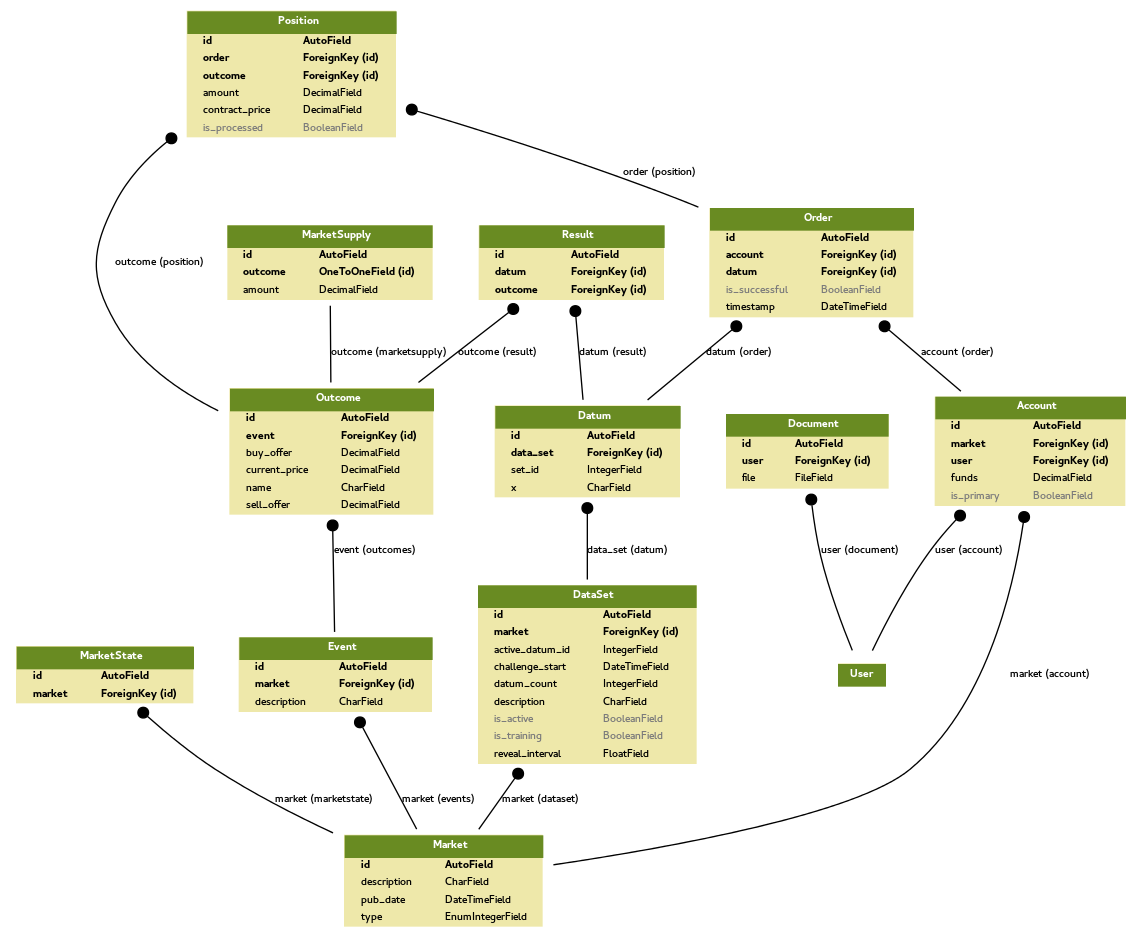
\includegraphics[scale=0.7]{markets_graph.png} }
\label{fig:class_diagram}
\caption{A class diagram of the models comprising the market core. }
\end{figure}


\subsection{Admin Interface}
    The admin interface is the place where market operator can create and configure the hosted markets and manage their contents (in terms of events and data sets) and state. 

	Since the framework comes with the built-in {\tt django-admin} module serving this exact purpose, implementing this interface was particularly straightforward. Thanks to the aforementioned module the most common and repetitive operations on models (i.e. create, read, update, delete) were purposefully easy to implement and configure. On the other hand other less ``popular" features, such as the option to pre-fill a dataset with randomised entries or to create both an event and its associated outcomes in one go, required carefully reading through the (often quite large) documentation.   

\subsection{API}
    
	Implementing a remote API was one of the more important features of the project in in terms of its intended use as a prediction market framework. Its basic premise is to allow for the development of automated agents that interact with existing markets. While in theory most if not all of its functionality mirrors that of the user interface, it is important that the API operates in a secure, well-defined fashion. 
    
    I first approached the problem by manually adding 
    
\section{Market Makers}
% talk about the market makers that were or can be implemented. 
    The following section 
	What follows is an overview of the created market maker interface and the pricing algorithms investigated in the scope of the project. 

\subsection{Interface}
	The two basic actions market makers should provide are processing orders and finalising challenges. 
	
\subsection{Order Book}
	
	The “city plaza” market scenario where potential buyers and sellers all place their bids and the matching buy/sell offers are resolved. There is normally more than one way to complete trades where for example an agent sells at a price lower than that of a matching buyer, or an agent wishes to buy a larger quantity than a seller has to offer. Usually the market maker is neutral towards both the goods and their prices, but can also be made active by e.g. resolving arbitrage opportunities in his favour.

	Although they are simple to implement and operate, auctions of this type tend to create thin markets with volatile prices and low liquidity of the assets being traded. We can furthermore use the concept of Nash Equilibria to show that such markets do not incentivise players to share their true beliefs and are thus not well suited for model estimation (Myerson et al. 1983). Consider for example a buyer who values a given good well above its current market price: he or she would have no incentive whatsoever to let others (“the market”) know about their high valuation of the good but will instead seek to make trades at the lower price.
	
\subsection{Parimutuel Betting}
This is the system usually used in gambling on sporting events, or in various lotteries. In it all bets of a type are put together in a pool, and the instantaneous odds are determined by the ratios between the already placed bets. The final winnings are determined by sharing the pool (minus any house cuts) amongst the winning bets. Although easy to implement and operate, such markets do not offer any guarantees on the amount to be won in case of success (i.e. the final odds) since the latter is not known until all bets are collected.

\subsection{Market Scoring Rule}
In a market scoring rule (MSR) prediction market agents report a probability estimate r on the outcomes of an event and are rewarded sci(r) when outcome i happens. Proper scoring rules are rules which reward estimates close to the truth the highest and penalise estimates that deviate from it, thus incentivising players to act according to their true beliefs.

 [TODO: Review] Such scoring rules are typically monotonically increasing, an example being sci(r)=a+bilog(ri) which is the logarithmic market scoring rule (log-MSR; Hanson, 2002). It is a proper scoring rule which quantifies the risk (also known as self-information in information theory) for the market maker at any time and charges participants proportionally to the change in risk their positions incur: players who move the market prediction towards the “true” distribution (or winning outcomes) get rewarded for doing so, while those who degrade the market prediction are penalised.

In general MSR market schemes are more involved than other examples but also allow for greater flexibility in the pricing strategies. 

\section{User Interface}
% mention the static interface, js graphics !!

	Due to my limited abilities in html and javascript the current user interface is fairly simple. Apart from basic features such as (secure) user registration and login it provides price quotes and transaction history for markets. There are a few directions I would like to expand on: for example by including histograms to visualise the prices or the trade volume in a market, by allowing browsing other agents’ portfolios, and making the interface more intuitive as a general. A great case study is presented in “A Combinatorial Prediction Market for the U.S. Elections” by Dudik et. al

\section{Other Tools}

\subsection{django-extensions}
    This package is an MIT-licensed collection of extension tools which ease the process of developing Django apps. Two most useful features I used were the ability to automatically generate {\tt django-admin} templates and GraphViz {\tt dot} files of the models in a package. The latter especially helped me visualise [TODO: Also does what?]

\subsection{Sphinx}
    Sphinx is a flexible documentation generator which converts {\tt reStructuredText} (reST) files to a number of formats, most notably PDF and HTML. ReST is a flexible markup language widely used for documentation purposes in the Python community. I was not initially supportive of the idea of learning yet another markup or template language but after looking at possible alternatives Sphinx looked like the most reliable, widely used and {\em pythonic} solution out there. In the end I was able to both quickly generate automatic documentation from the code, and then manually extend and insert additional explanations and use cases for the examples in question. 

\section{Testing and Documentation}
% documentation at github.io ?!
% issue tracker ?!?!
% wiki too ?!?!?!?
	When it comes to designing and testing an application dealing with any kind of transactions, it is clear that a set of minimum requirements has to be met in terms of consistency and transaction atomicity. Fortunately the high-level nature of the language and the framework make this straightforward. 

	I initially wanted to adopt a test-driven approach towards units tests but doing so proved hard for the first few months of the project. Since it is straightforward to introduce runtime validation or assertions in Python I used that extensively from the start. During that time I was mainly modelling the market structure and writing code for the front-end. Most of the work was thus of declarative nature and needed little, if any, tests. 
	I followed a similar approach with documentation by providing extensive {\tt AutoDoc} comments inside the code for the most of the project. I found   

\subsection{Unit Tests}

	The testing process was not without its quirks related to the framework I used. After I completed the first few tests and proceeded to run them I noted they were all failing in a very specific way: although I could create objects in the test database and manipulate them referentially, accessing them using query selectors inevitably failed. could find more test targets in terms of functionality. This allowed me to statically verify some of the assertions made 
	
	While I was implementing the market makers I 
	
\subsection{Runtime Tests}
    
    The code features a multitude of runtime tests checking model invariants. For example the joint asset prices for an outcome space always summing to 1 is enforced throughout the market makers, but there are also explicit checks executed every time prices change.

    While designing the base models I paid extra attention to transaction atomicity: it would be quite inappropriate if funds appeared or vanished while serving requests in a market. Thankfully the framework makes implementing this easy and idiomatic enough so I had no problems accomplishing it using method decorators and with blocks.

\subsection{Documentation}

    The documentation is an integral part of the life-cycle of any extensible and maintainable software and that is especially true in the case of a framework of any kind. For the most of my time working on the project I was relying on 
    
\subsection{Issues}
    As I was using the 
    
\chapter{Evaluation/Reflection}

\section{Functionality}

\chapter{Conclusion}
	Prediction markets have already been studied for a while. Nonetheless there are 
% its a stepping stone for creating advanced prediction markets. Hopefully not rough. 




% use the following and \cite{} as above if you use BibTeX
% otherwise generate bibtem entries
\bibliographystyle{unsrt}
\bibliography{ixlib}

\end{document}
